\documentclass[11pt,a4paper]{article}
\usepackage[margin=1.0in]{geometry}
\usepackage{setspace}
\doublespacing
\usepackage{enumitem}
\usepackage{url}
%%%%%%%%%%%%%%%%%%%%%%%%%%%%%%%%%%%%%%%%%%%%%%%%%%%%%%%%%%%%%%%%
%% Graphicx.sty for Including PostScript .eps files
\usepackage{graphicx}
\usepackage{epstopdf}
%%%%%%%%%%%%%%%%%%%%%%%%%%%%%%%%%%%%%%%%%%%%%%%%%%%%%%%%%%%%%%%%
\begin{document}

%% Title Pages
%% Setting up title pages, type in the appropriate names here:
\title{CBC Test Software Instructions \\ version 0.01}

\author{Kirika Uchida\\
	k.uchida@imperial.ac.uk}
	%or
	%\authors{}

	\maketitle
	\tableofcontents
	\listoffigures %optional
	\listoftables  %optional

	\section{Introduction}
	The CMS Binary Chip 2 (CBC2) amplifies signals from sensors to create binary hit information at the comparator, 
	based on the signal input and the threshold voltage. 
	Those voltages have to be adjusted to achieve good efficiency of hits from signals with sufficiently low noise rate. 
	This is achieved through adjusting three register settings on the CBC2: VPLUS, OFFSETs, and VCTH.  
	VPLUS tunes the DC signal voltage at output of the postamp and VCTH sets the comparator threshold voltage for all the channels in the chip.  
	The OFFSETs are used for fine tuning of the DC voltage for the 254 channels individually. 
	Constraints on those register values from the hardware requirements and 
	proposed calibration sequence are explained in Chapter \ref{ch:architecture-proposal}, 
	and the implementation of the software in the beamtest setup are detailed in Chapter \ref{ch:implementation}.  

	\section{CBC2 architecture and calibration proposal}\label{ch:architecture-proposal}
	\subsection{Registers for calibration}\label{sec:reg}
	The simplified CBC2 schematic is shown in Figure \ref{fig:CBC2} with the signal shapes at each point.  
	The registers VPLUS and VCTH have the same range of voltage setting as shown in Figure \ref{fig:volt-i2c}. 
	These registers are global in the CBC2 and VPLUS should be high (low) enough to cover the signal range for electron (hole) mode.
	While the register OFFSETs are set for individual signal channels. 
	The OFFSET registers are for fine tuning of the postamp output, adjusting the current flow in Figure \ref{fig:CBC2}. The OFFSET values should not be too close to zero. 

	\begin{figure}[htbp]
	\centering
	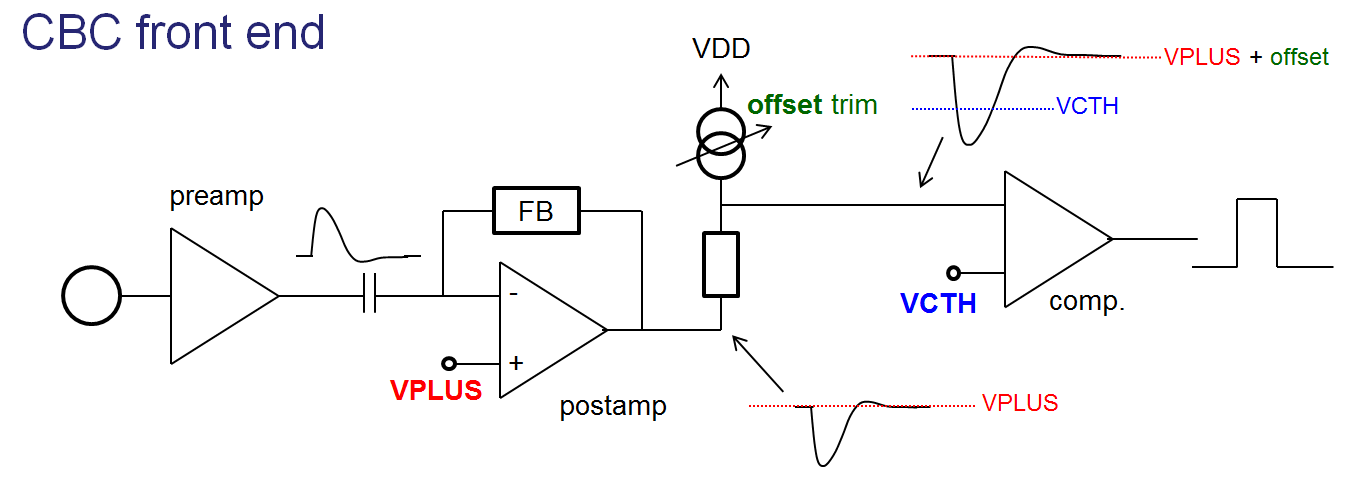
\includegraphics[width=\textwidth]{fig/CBC.png}
	\caption{Simplified CBC2 schematics and signal pulse shape for electron mode. }\label{fig:CBC2}
	\end{figure}

	\begin{figure}[htbp]
	\centering
	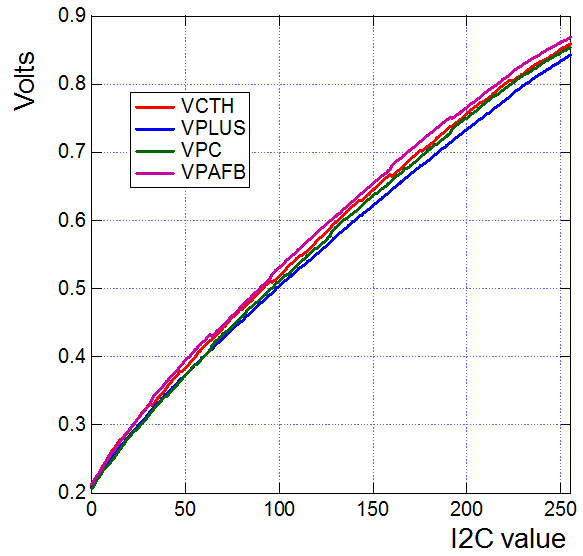
\includegraphics[width=0.5\textwidth]{fig/VoltI2c.png}
	\caption{Voltage vs. register value. }\label{fig:volt-i2c}
	\end{figure}

	\subsection{Calibration strategy}
	Calibrating the CBC2 results in setting the signal efficiency and noise rate.
	Tuning involves data taking and hit rate calculation in different CBC2 register settings. 
	A threshold (VCTH) scan over different register values gives an s-curve in a 2D space: hit rate vs. VCTH.
	A calibration aligns the s-curves of all the channels so that the 0.5\% hit rate point corresponds to
	a certain VCTH value (the VCTH middle point) by tuning OFFSETs for all the channels. 
	Depending on the condition of the VCTH scan, either an efficiency of a certain charge deposit or a noise rate
	for all the channels can be obtained. 

	To calibrate the CBC2, an s-curve alignment is done with a certain number of test pulses created inside CBC2.  This approach was chosen not to fire too many channels all together during
	the VCTH scan which causes too much load on the comparator. A maximum of 32 channels are fired in this method since test pulses are generated for 32 channels.
	However, it is not easy to estimate the effect of inaccuracy in size and timing jitter of the test pulses.
	Therefore, another strategy is proposed where s-curve alignment is done without the test pulse, overcoming the over loading problem. 
To fire only certain number of channels, OFFSETs for channels which are not under calibration are set to the maximum (minimum) value for electron (hole)
	mode.  In this way, s-curves on target channels are obtained in the range where other channels are not fired as shown in Figure \ref{fig:pedestals}.

	\begin{figure}[htbp]
	\centering
	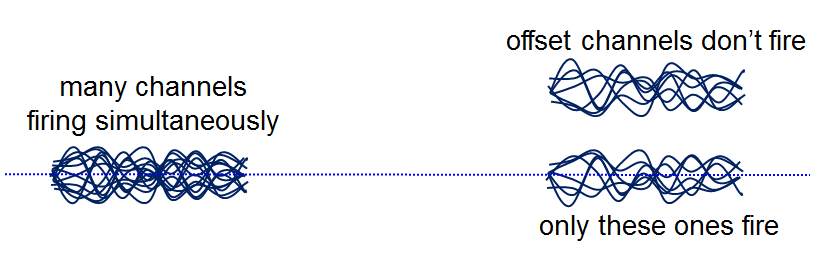
\includegraphics[width=\textwidth]{fig/pedestals.png}
	\caption{Pedestals for channels under calibration and others. }\label{fig:pedestals}
	\end{figure}

	\subsection{Calibration sequence}\label{subsec:calib-sequence}

	The first step is to find a reasonable value for target VCTH middle point for pedestal s-curve.  
The voltage set by VCTH corresponds to the voltage set by VPLUS $+\alpha$(from OFFSET) 
	and this value has to be high (low) enough to cover the signal range for electron (hole) mode.
	There is a requirement on the OFFSETs not to be close to zero as discussed in \ref{sec:reg}. 
	It was found that the relation between offset voltage and OFFSET register value is 
	linear with small variation of the slope over the channels due to the resister variation over channels as shown in Figure \ref{fig:offset-i2c}.
	This is speculated from a study where OFFSET value distribution from an s-curve alignment with different target VCTH middle point also as shown in Figure \ref{fig:offset-i2c}. It is concluded that the OFFSETs should be non zero and in a good range to be able to adjust the comparator input voltage. To satisfy these requirements, the following sequence is proposed. 

	\begin{itemize}
	\item Set target VCTH middle point value to 120.
	\item Perform VCTH scan and obtain s-curves setting all OFFSETs to 80 for some VPLUS values.
	\item Obtain VPLUS value which corresponds to average VCTH middle point to be 120. 
	\item Perform s-curve alignment with the VPLUS with the target VCTH middle point.
	\end{itemize}

	This procedure should give the OFFSETs distribution around 80 and a reasonable VPLUS value.

	\begin{figure}[htbp]
	\centering
	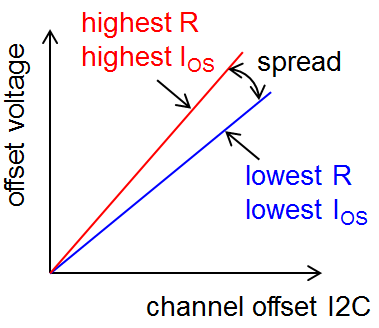
\includegraphics[width=0.4\textwidth]{fig/OffsetI2c.png}
	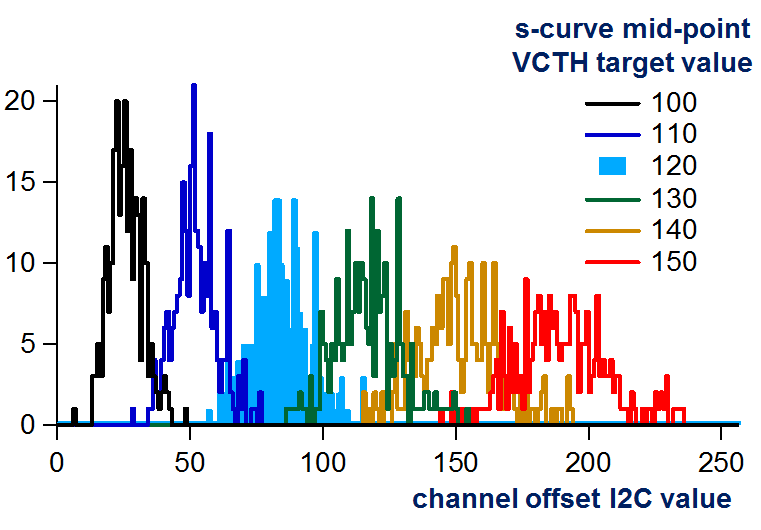
\includegraphics[width=0.55\textwidth]{fig/VcthMidI2c.png}
	\caption{Offset vs. register value on the left and OFFSET value distribution from s-curve alignment with different target VCTH middle points. }\label{fig:offset-i2c}
	\end{figure}

	\section{Implementation}\label{ch:implementation}
	A software package, CbcTest is prepared for the proposed calibration in the previous section.
	The VCTH scans are done for each group of channels one by one, where channels are grouped in the same as the test pulse group.
	The software creates CBC register setting files with the calibrated register values and ROOT files which contain histograms 
	and the fit functions for s-curves in each step of the calibration.

	\subsection{Hardware setup}
	A testbench is set up in a similar environment as the beamtest in 2013 at DESY with a backend GLIB\cite{GLIB} board and a frontend board with 2 CBC2 chips connected to a FMC on the GLIB.
	Figure \ref{fig:testbench} shows the diagram of the setup.  A firmware loaded on the FPGA on the GLIB is tracker1.2glibv3.dualcbc2.r123 (Strasbourg's firmware)\cite{FIRMWARE}.  FMC have to be connected to J1 with this firmware.

	\begin{figure}[htbp]
	\centering
	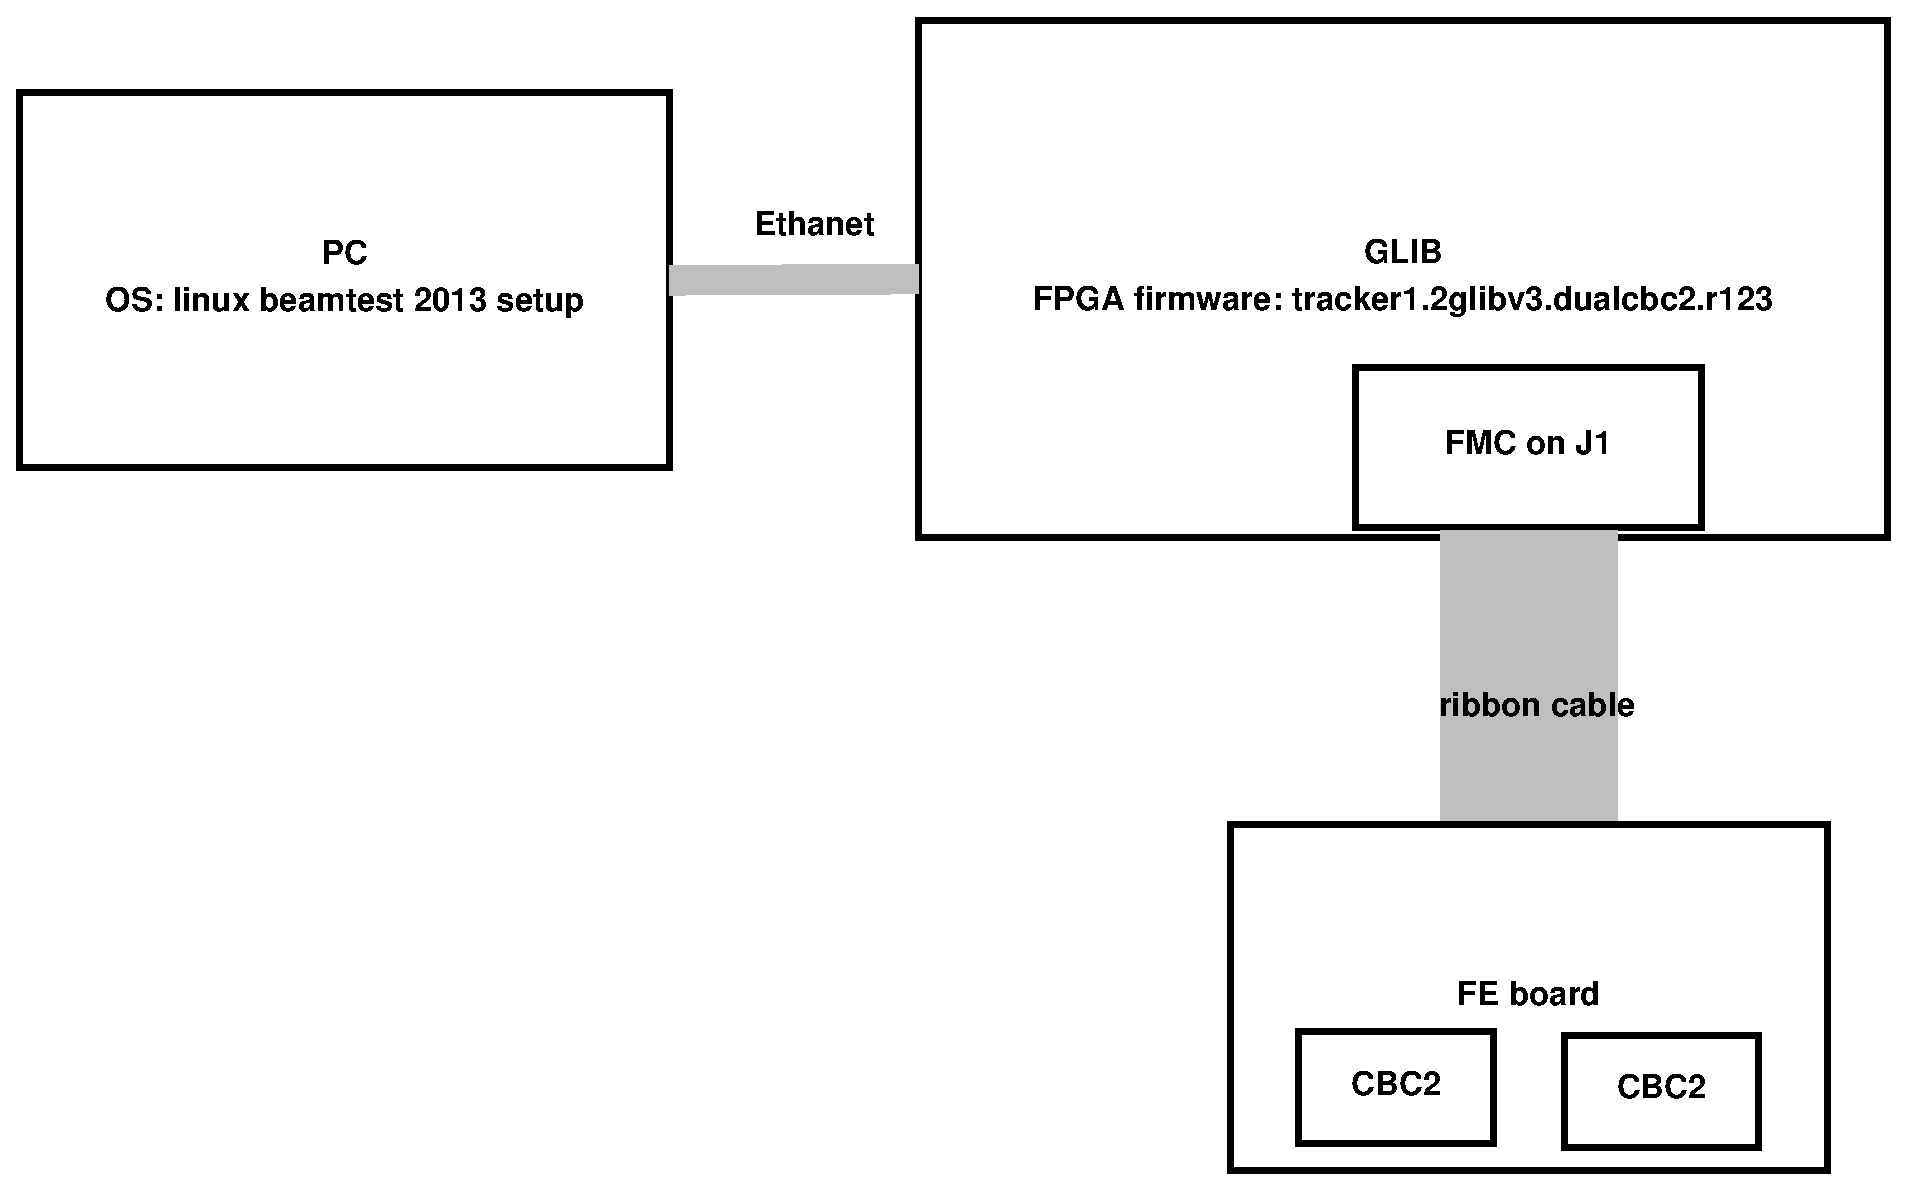
\includegraphics[width=\textwidth]{fig/TestBench.eps}
	%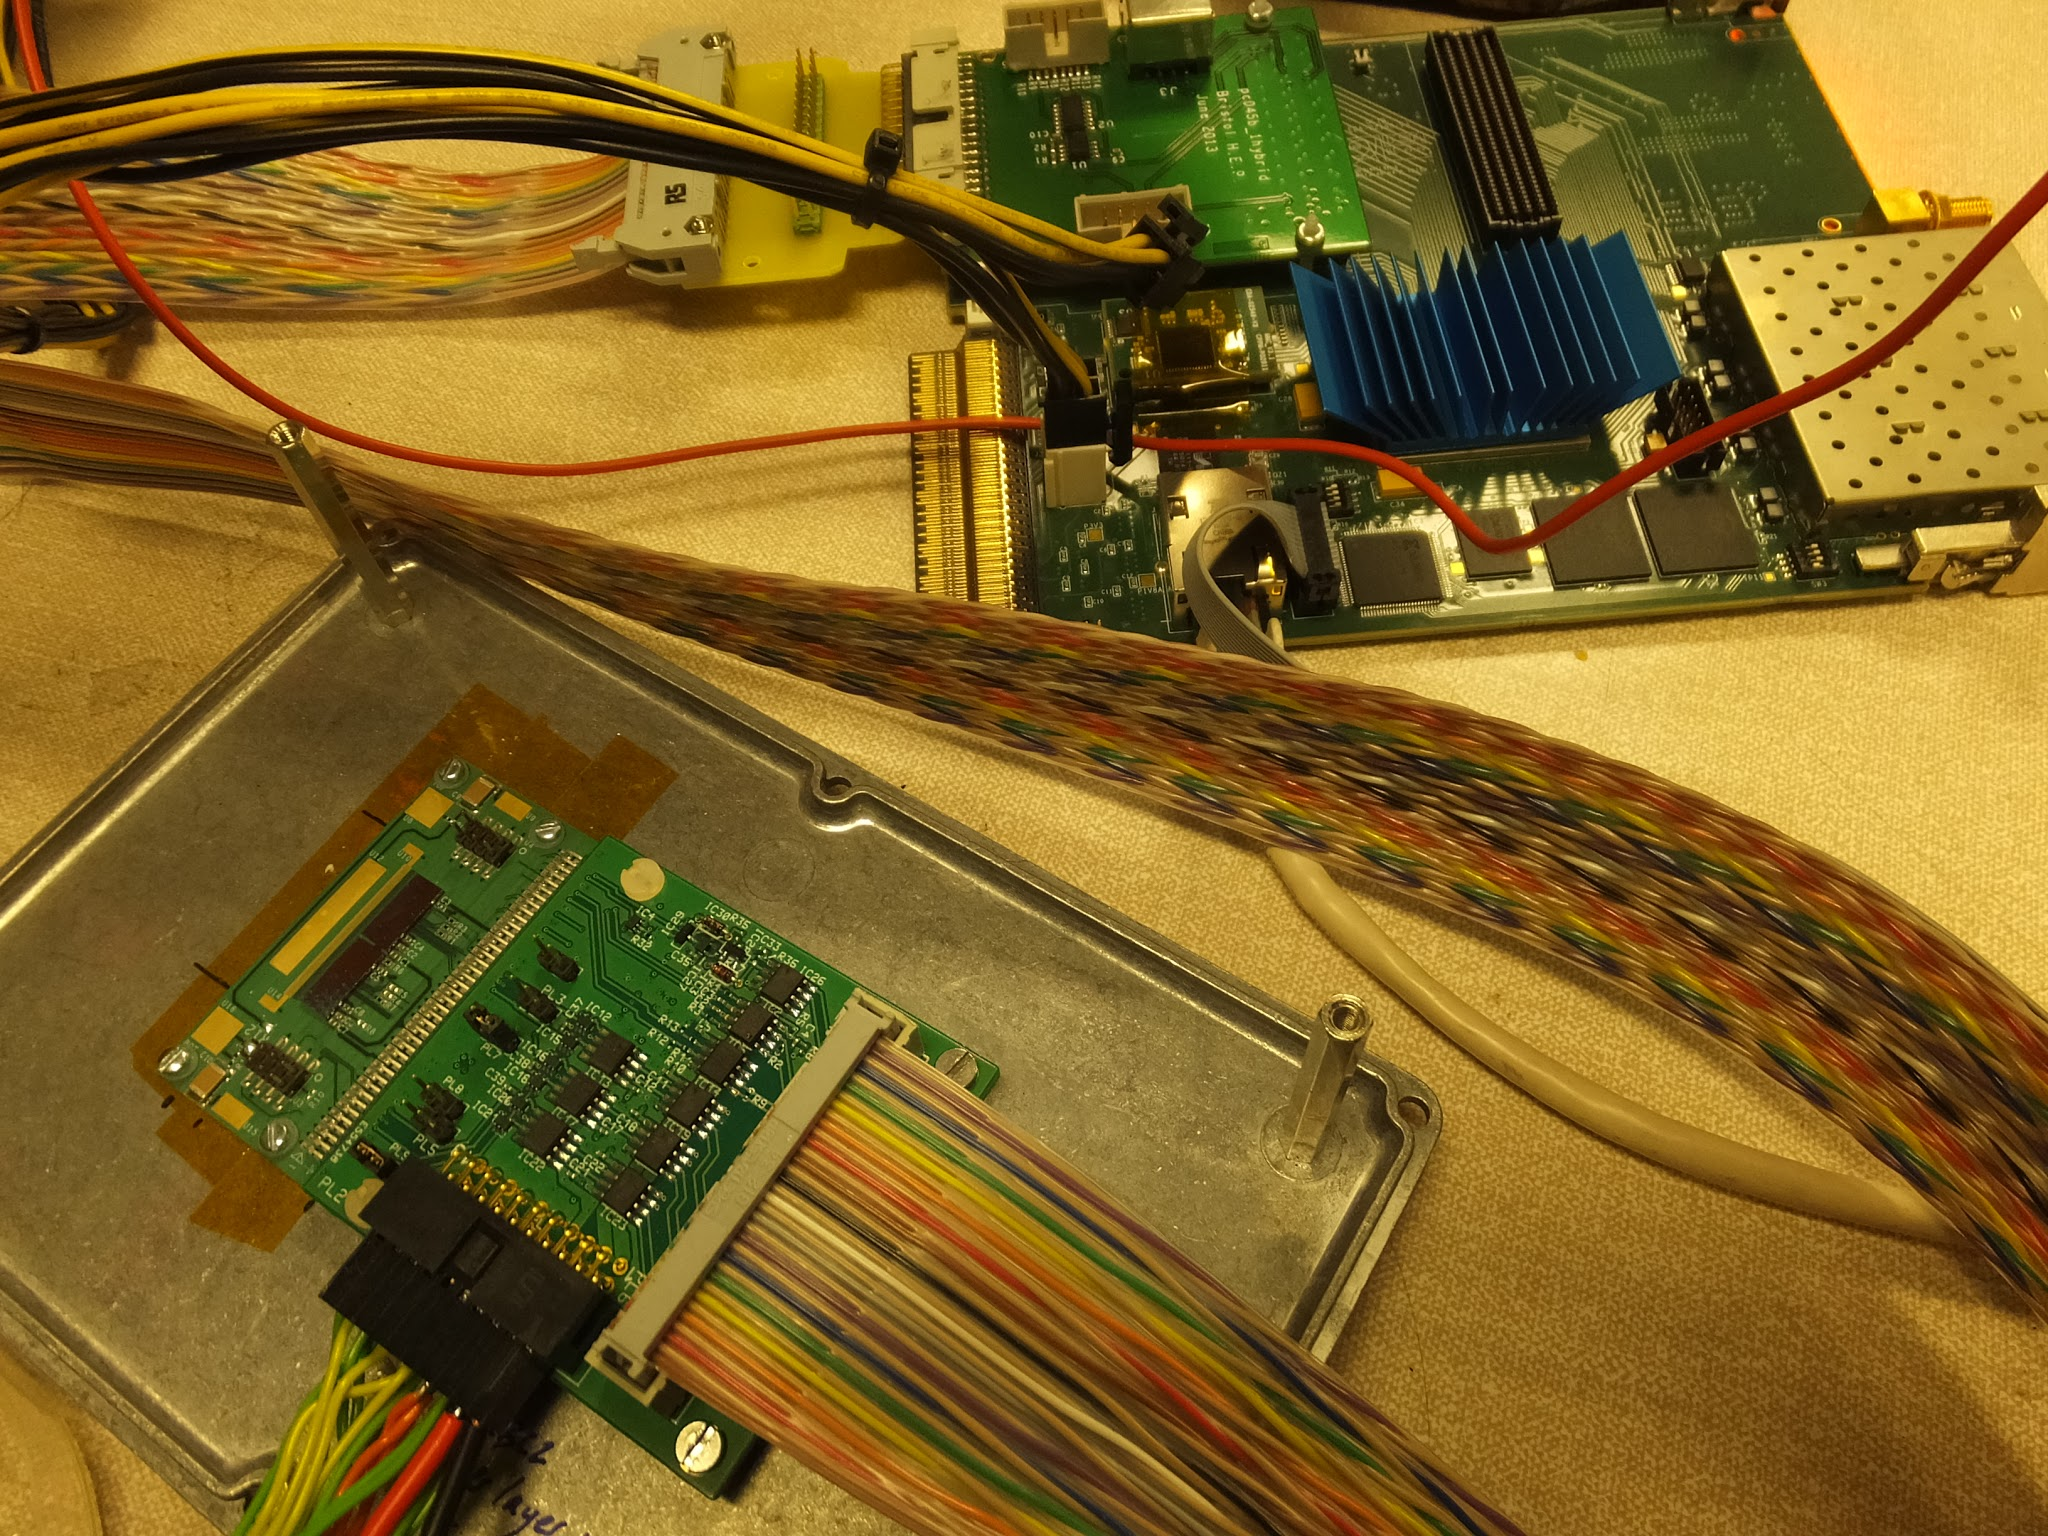
\includegraphics[width=\textwidth]{fig/TestBench.jpg}
	\caption{Testbench diagram. }\label{fig:testbench}
	\end{figure}

	\subsection{Software package: CbcTest}
	The software is coded in C++ using UHAL\cite{UHAL} for the hardware interface (IPBUS) and ROOT\cite{ROOT} is used mainly for histograming and the GUI. 
	This is built as a standalone software outside the beamtest DAQ but no additional library is required. The software package is named CbcTest and located at SVN\cite{CBCTEST}. 

	\subsubsection{Structure}
	The CbcTest packages is provided in a compressed tar file, CbcTest.tgz on SVN. Files are extracted with the top directory CbcTest. 
	The CbcTest consists of {\it setup.sh} for environment setting, {\it Makefile} for building, and 10 directories.  
	Four of the directories, {\it utils, Cbc, Strasbourg, and ICCalib} contain source files for each library and the compiled libraries are installed under {\it lib}.
{\it utils} has some useful tools, {\it Cbc} defines classes of structured CBC register data instances, {\it Strasbourg}  is for the interface with Strasbourg's firmware, {\it ICCalib} contains the proposed calibration sequence and GUI interface.  
{\it src} has calibration and VCTH scan source codes for CUI and GUI using the libraries and executables are built and installed under {\it bin}. 
{\it settings} directory contains some calibration and CBC register settings and {\it macros} directory has some useful ROOT macros for the calibration output root files. 
In the last, {\it doc} directory is for this documentation.   

\subsection{User guide}

\subsubsection{Setup and build}

At the top directory, execute the following commands at bash shell prompt, 
   \begin{quote}
   \verb|source setup.sh|\\
	   \verb|make|
	   \end{quote}
	   After the make, executables are created under bin. In the default setting, the executables are expected to be invoked at the top directory.
	   This is just because the default path for input setting files are set to the relative path \verb|./settings/...|.  The input path can be given as an option
	   in CUI and changed in GUI.

	   \subsubsection{Input setting file}
	   As seen in settings/CbcCalibElectron.txt, the setting file consist of lines with variable name and the value separated by ":".
	   The explanations of the variables are as follows,

	   \begin{description}[style=nextline]
	   \item[GlibConfigurationFile] xml connection file for ipbus.
	   \item[GlibBoardId] the board id in the xml connection file. 
	   \item[BeId] backend board id, used for output directory and histogram names for multiple GLIB settings. 0 or positive number is expected.
	   If this is not given, 0 is used in the software.
	   \item[GlibReg\_CBC\_expected] 1 for 1 CBC and 3 for 2 CBC
	   \item[GlibReg\_COMMISSIONNING\_MODE\_CBC\_TEST\_PULSE\_VALID] Commissioning mode and make test pulse enabled (disabled) on GLIB for 1 (0).
	   \item[GlibReg\_COMMISSIONNING\_MODE\_DELAY\_AFTER\_FAST\_RESET] Number of clock cycle to wait for the GLIB to send signal to the CBC to generate test pulse after FAST RESET.
	   \item[GlibReg\_COMMISSIONNING\_MODE\_DELAY\_AFTER\_TEST\_PULSE] Number of clock cycle to wait for the GLIB to send L1A to the CBC after sending signal to the CBC to generate test pulse.
	   \item[GlibReg\_COMMISSIONNING\_MODE\_DELAY\_AFTER\_L1A]        Number of clock cycle to wait for the  GLIB to send FAST RESET to the CBC after L1A.
	   \item[GlibReg\_COMMISSIONNING\_MODE\_RQ] GLIB COMMISSIONING MODE request. 1 for calibration data acquisition.
	   \item[GlibReg\_FE\_expected]                                Number of the frontend board.   1 (3) for 1 (2) board.
	   \item[GlibReg\_user\_wb\_ttc\_fmc\_regs.pc\_commands.CBC\_DATA\_PACKET\_NUMBER] Number of event per acquisition.
	   \item[GlibReg\_user\_wb\_ttc\_fmc\_regs.pc\_commands2.negative\_logic\_CBC] 1 (0) for electron (hole) mode.
	   \item[GlibReg\_cbc\_stubdata\_latency\_adjust\_fe1]
	   \item[GlibReg\_cbc\_stubdata\_latency\_adjust\_fe2]         
	   \item[GlibReg\_user\_wb\_ttc\_fmc\_regs.pc\_commands.ACQ\_MODE]
	   \item[GlibReg\_user\_wb\_ttc\_fmc\_regs.pc\_commands.CBC\_DATA\_GENE] 
	   \item[GlibReg\_user\_wb\_ttc\_fmc\_regs.pc\_commands.INT\_TRIGGER\_FREQ]
	   \item[GlibReg\_user\_wb\_ttc\_fmc\_regs.pc\_commands.TRIGGER\_SEL]
	   \item[GlibReg\_user\_wb\_ttc\_fmc\_regs.pc\_commands2.clock\_shift]
	   \item[GlibReg\_user\_wb\_ttc\_fmc\_regs.pc\_commands2.negative\_logic\_sTTS]
	   \item[GlibReg\_user\_wb\_ttc\_fmc\_regs.pc\_commands2.polarity\_tlu]
	   \item[CbcConfig\_FE0CBC0] CBC register settings file for front end board id 0 and CBC id 0 
	   \item[CbcConfig\_FE0CBC1] CBC register settings file for front end board id 0 and CBC id 1 
	   \item[Calib\_InitialOffset] Initial OFFSET value for offset calibration. Leave it to 0x00. The value has to be written in hexadecimal.
	   \item[Calib\_TargetOffset] The target OFFSET value. 0x50 as default. The value has to be written in hexadecimal.
	   \item[Calib\_TargetVCth]   Target VCTH value.  0x78 as default. The value has to be written in hexadecimal.
	   \item[Calib\_VplusMax.]    VPLUS maximum value to scan. 0x90 as default. The value has to be written in hexadecimal.
	   \item[Calib\_VplusMin.]    VPLUS minimum value to scan. 0x60 as default. The value has to be written in hexadecimal. 
	   \item[Calib\_VplusStep]    VPLUS scan step value. 0x10 as default. The value has to be written in hexadecimal.
	   \end{description}

	   Do not change the variables which are not explained above.

	   \subsubsection{calib}

	   \verb|USAGE: calib ( [mode] [setting filename] )|\\
		   The [mode] is either {\it electron} or {\it hole}.
		   If [mode] is not given, electrom mode is invoked. If [setting filename] is not given, 
		   the files under ./settings, CbcCalibElectron.txt (CbcCalibHole.txt) for electron (hole) mode.
		   If those files do not exist, the application still runs with the default setting found in DAQController.cc
		   This command executes the procedure explained in Section \ref{subsec:calib-sequence}.

		   \subsubsection{vcthscan}

		   \verb|USAGE: vcthscan ( [mode] [potentiometer value] [setting filename] )|\\
			   The [mode] is either {\it electron} or {\it hole}.
	If [mode] is not given, electron mode is invoked. 
If [potentiometer value] is not given, -1 is set (no test pulse)
	If [setting filename] is not given, 
	the files under ./settings, CbcCalibElectron.txt (CbcCalibHole.txt) for electron (hole) mode.
	If those files do not exist, the application still runs with the default setting found in DAQController.cc

	This command scans VCTH and creates the s-curves with all the other registers fixed except for the case when test pulse is disabled. 
	If the test pulse is disabled, the scan is also done for group by group and the same trick is made for other OFFSETs as in the calibration. 

	\subsubsection{calibGUI}

	\verb|USAGE: calibGUI|\\
		calibGUI consists of the configuration file setting frame on top, command buttons on the bottom, and seven tabs in the middle, [DAQ\&GLIB configuration], [Log], [CBC register], 
	[Calibration configuration] [Vplus vs. VCth0 Graphs], [Scurve Histograms], and [Data].
	The configuration file can be changed anytime. Write down the file path in the text field and push [Load] button.  Recommended buttons to proceed to the next step are highlighted in orange colour. Other valid command buttons are also accessible if you want.
	The normal sequence is to press "ConfigureGlib", "ConfigureCbc", ConfigureCalibration", in the order and either press "Calibrate" or "VCthScan" after that.
	"Calibrate" executes the procedure explained in Section \ref{subsec:calib-sequence}.
	"VCthScan" scans VCTH and creates the s-curves with all the other registers fixed except for the case when test pulse is disabled. 
	If the test pulse is disabled, the scan is also done for group by group and the same trick is made for other OFFSETs as in the calibration. 
	It is better not to move the top window when the calibration is on going to avoid the ROOT to crash.
	Each tabs are explained as follows.
	\begin{description}[style=nextline]
	\item[DAQ\&GLIB configuration] 
	The GLIB address and ID, and GLIB register values are customised in this tab on the fly. Press "ConfigureGlib" to configure glib after modifying the values in the fields. After the GLIB is configured, CBC register setting files set in the configuration file (default values if not set in the setting file) are shown in the left and "ConfigureCBC" button is highlighted. Those can be modified before pressing "ConfigureCBC" button. 
	\item[Log]
	Log is shown in this tab.
	\item[CBC register]
	After pressing "ConfigureCbc" button, the register configuration from the files shown in the 
	[DAQ\&GLIB configuration] tab appear in this tab. Each Front end (FE) tab contains it's own CBC tabs. 
	Each CBC tab has it's setting file name field and this can be modified and "LoadAndSet" button load the settings file and those values are set to the CBC register and the result is shown in the GUI panel.
	All the CBC register values are customised on the fly. 
	Registers in Page 1 are listed with the name, address, the read back value after writing the value to the register in the CBC, and the written value from the left to the right.  
	Registers in Page 2 are listed in the same way but without the name. The right most field is editable.  
	If the arrow is clicked or pressed enter after modifying the value, GUI recognises that those are changed and background color changes to orange.  
	You can edit as many field as you want for all the CBCs at the same time. 
	"UpdateCbcRegisters" button at the top of the [CBC register] tab is to write the values to CBCs and GUI panel is updated.
	If the read back value is different from the set value, the field color turns to red, otherwise returned to white.
	"Reset" button next to the "UpdateCbcRegisters"  resets all the modification made and orange highlights and the values are reset.
	Current CBC register values can be saved with "Save" button next to "LoadAndSet" button in each CBC tab.  
	The file name in the editable file name field is used as the output file name. Please change the file name if you do not want to overwrite the file.

	\item[Calibration configuration]
	Calibration configuration is customised in this tab before pressing "ConfigureCalibration".  
	EnableTestPulse can be set to 1 for VCthScan. This is ignored in Calibration.

	\item[Vplus vs. VCth0 Graphs]
	This tab shows Vplus vs. VCth0 graphs in the step to obtain Vplus value in the calibration. 

	\item[Scurve Histograms]
	All the s-curves from VCTH scan are shown in this tab.

	\item[Data]
	If "Start data stream display" button is pressed, prescaled data stream is shown in this tab.  This slows down the procedure and can be disabled
	any time by clicking "Stop data stream display".

	\end{description}

	\bibliography{CMS_UPGRADE}
	\bibliographystyle{plain}
	\end{document}

